%md->tex->template
\documentclass[12pt]{article}
\usepackage{CJKutf8}
\usepackage{amsmath}
\usepackage{geometry}
\usepackage{fancyhdr}
\usepackage{longtable,booktabs}
\usepackage{enumerate}
\usepackage{enumitem}
\usepackage{amsthm}
\usepackage{amssymb}
\usepackage{tikz}
\setlist[enumerate,1]{font=\bfseries}
\geometry{left=3.0cm,right=2.0cm,top=3.0cm,bottom=3.0cm}

\newenvironment{firstlayer}%
{\begin{list}{}{\renewcommand{\makelabel}[1]{\textbf{##1}.\hfil}
}}
{\end{list}}
\newenvironment{secondlayer}%
{\begin{list}{}{\renewcommand{\makelabel}[1]{(##1)\hfil}
}}
{\end{list}}

\renewcommand{\proofname}{\textbf{证明}}

\providecommand{\sol}{\textbf{解}.~}

\title{第 14 次作业}
\author{Log Creative}
\date{June 13, 2020}
\begin{document}

\begin{CJK}{UTF8}{gbsn}

\maketitle

\begin{firstlayer}
  \item[习题一]
  \begin{firstlayer}
    \item[2]简单图$G$中,如果$m>\frac{1}{2}(n-1)(n-2)$,证明$G$不存在孤立节点。
    \begin{proof}
      若不然,则有一孤立点$v$,子图$G'=G-v$的边数
      \begin{equation}\label{ls}
        \mid E(G')\mid =\mid E(G)\mid=m>\frac{1}{2}(n-1)(n-2)
      \end{equation}
      
然而,$G'$边数最多的情况是完全图$K_{n-1}$,也就是
\begin{equation}\label{lss}
  \mid E(G')\mid \leq \frac{1}{2}(n-1)(n-2)
\end{equation}

这与式子(\ref{ls})矛盾。

由于当孤立节点数不止一个时,式子(\ref{lss})依然成立。所以不存在孤立节点。

    \end{proof}
    \item[3]完全图的每边任给一个方向,称为有向完全图。证明在有向完全图中
\begin{equation}\label{3p}
  \sum_{v_i\in V}(d^+(v_i))^2 = \sum_{v_i\in V}(d^-(v_i))^2
\end{equation}

\begin{proof}
  注意到,在完全图$K_n$中,所有节点的度数都是$n-1$,则:
\begin{align}
    &\sum_{v_i\in V}(d^+(v_i))^2 - \sum_{v_i\in V}(d^-(v_i))^2 \nonumber\\
=&\sum_{v_i\in V} \left[(d^+(v_i))^2 - (d^-(v_i))^2\right]\nonumber\\
=&\sum_{v_i\in V}(d^+(v_i)+d^-(v_i))(d^+(v_i)-d^-(v_i))\nonumber\\
=&\sum_{v_i\in V}d(v_i)(d^+(v_i)-d^-(v_i))\nonumber\\
=&\sum_{v_i\in V}(n-1)(d^+(v_i)-d^-(v_i))\nonumber\\
=&(n-1)\left[\sum_{v_i\in V}d^+(v_i)-\sum_{v_i\in V}d^-(v_i)\right]
\end{align}

对于每一条有向边来说,在这一个顶点产生了出度,必定会在另一个顶点产生入度,那么顶点的出度总数与入度总数将是相同的,所以:
\begin{equation}
  \sum_{v_i\in V}(d^+(v_i))^2 = \sum_{v_i\in V}(d^-(v_i))^2
\end{equation}

\end{proof}

\item[8]写出图1.7(a)中的邻接矩阵和关联矩阵。

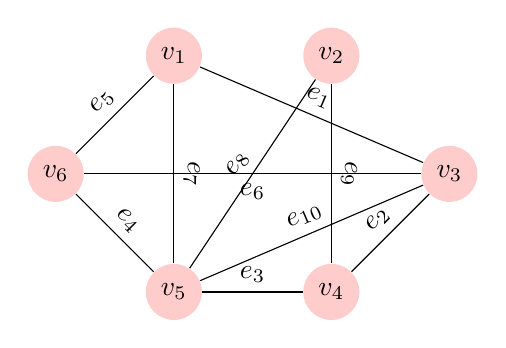
\begin{tikzpicture}

\node[circle,fill=red!20] (v1) at (-1.5,2.5) {$v_1$};
\node[circle,fill=red!20] (v2) at (0.5,2.5) {$v_2$};
\node[circle,fill=red!20] (v3) at (2,1) {$v_3$};
\node[circle,fill=red!20] (v4) at (0.5,-0.5) {$v_4$};
\node[circle,fill=red!20] (v5) at (-1.5,-0.5) {$v_5$};
\node[circle,fill=red!20] (v6) at (-3,1) {$v_6$};

\draw  (v1) edge node[above,sloped] {$e_1$} (v3);
\draw  (v3) edge node[above,sloped] {$e_2$} (v4);
\draw  (v4) edge node[above,sloped] {$e_3$}(v5);
\draw  (v5) edge node[above,sloped] {$e_4$}(v6);
\draw  (v6) edge node[above,sloped] {$e_5$}(v1);
\draw  (v6) edge node[below,sloped] {$e_6$}(v3);
\draw  (v1) edge node[above,sloped] {$e_7$}(v5);
\draw  (v2) edge node[above,sloped] {$e_8$}(v5);
\draw  (v2) edge node[above,sloped] {$e_9$}(v4);
\draw  (v3) edge node[above,sloped] {$e_{10}$}(v5);

\end{tikzpicture}

\sol 邻接矩阵

\begin{equation}
  A=\left(\begin{matrix}
    0 & 0 & 1 & 0 & 1 & 1 \\
    0 & 0 & 0 & 1 & 1 & 0 \\
    1 & 0 & 0 & 1 & 1 & 1 \\
    0 & 1 & 1 & 0 & 1 & 0\\
    1 & 1 & 1 & 1 & 0 & 1\\
    1 & 0 & 1 & 0 & 1 & 0
\end{matrix}\right)
\end{equation}


关联矩阵
\begin{equation}
  B=\left(\begin{matrix}
    1 & 0 & 0 & 0 & 1 & 0 & 1 & 0 & 0 & 0\\
    0 & 0 & 0 & 0 & 0 & 0 & 0 & 1 & 1 & 0\\
    1 & 1 & 0 & 0 & 0 & 1 & 0 & 0 & 0 & 1\\
    0 & 1 & 1 & 0 & 0 & 0 & 0 & 0 & 1 & 0\\
    0 & 0 & 1 & 1 & 0 & 0 & 1 & 1 & 0 & 1\\
    0 & 0 & 0 & 1 & 1 & 1 & 0 & 0 & 0 & 0
\end{matrix}\right)
\end{equation}

  \end{firstlayer}
  \item[习题二]
  \begin{firstlayer}
    \item[2]证明$G$和$\bar{G}$至少有一个是连通图。
    
    \begin{proof}
      不失一般性,设$G$是非连通图,则$G$中存在极大连通子图$S\neq G$。对于所有的节点$v_i\in S$,由于$\bar{G}=K_n-G$,则在$\bar{G}$中,$v_i$将与$\forall v_j\in G-S$相连。
      
      这样,纵使最坏情况,$\bar{G}$中关于$v_i\in S$的支撑子图和$v_j\in G-S$的支撑子图都是不连通的,但是两个点集所对应的点对$(v_i,v_j)$都有边相联系,则$\bar{G}$是连通的,事实上,在这种最坏情况下,$\bar{G}$为二分图。

反之亦然。
    \end{proof}
    
    \item[3]证明连通图有的最长道路必定相交于同一节点。
    
    \begin{proof}
      若只有一条最长道路,则自己与自己必然相交。下面证明非平凡的情况:

若不然,假设有两条等长的最长道路$P_1=(a_1,\cdots,a_n)$和$P_2=(b_1,\cdots,b_n)$,两者不相交。由于图是连通的,则必然有$a_1$到$b_1$的路径连接,设为$P_3=(a_1,c_1,\cdots,c_r,b_1)$,那么$P'=(a_1,c_1,\cdots,c_r,b_1,\cdots,b_n)$比两者都长(长度至少为$n$,大于$n-1$),矛盾!

故连通图有的最长道路必定相交于同一节点。
    \end{proof}
  \end{firstlayer}
\end{firstlayer}


\end{CJK}

\end{document}

